DVMS~\cite{quesnel:cpe2012} (Distributed Virtual Machine
Scheduler) is a framework that schedules VMs cooperatively and dynamically in
large-scale distributed systems.

\subsubsection{Overview and Definitions}
From a software point of view, the nodes are organized following a ring
topology.

A scheduling procedure is started as soon
as an event occurs on the infrastructure.

Each event is associated with a partition.  A partition is composed of all the
nodes that are reserved for the resolution of a specific event.
%
Partitioning the infrastructure is mandatory to avoid conflicts between several
schedulers that could manipulate the same nodes or VMs when they apply their
reconfiguration plans.

Each partition includes two special nodes, the initiator and the leader.
The initiator of a partition is the node that
initially produced the event associated with this partition.
The leader of a partition is the node that leads the scheduling computations
aiming at solving the event associated with this partition; the leader of
the partition is likely to change during the processing of the event.


\subsubsection{The Problem Solving Procedure}

The problem solving procedure is initiated when a node
N\(_{\textit{i}}\) observes that there is a problem, for instance when its
resources are overused (see Figure~\ref{fig:dvms_pte}); it then generates an
event and reserves itself to process this event (see
Figure~\ref{fig:dvms_pte_1}).  After that, it forwards this event to its
neighbor on the ring, node N\(_{\textit{i+1}}\).

If N\(_{\textit{i+1}}\) is already involved in another partition, it directly
forwards the event to node N\(_{\textit{i+2}}\); otherwise, N\(_{\textit{i+1}}\)
joins the new partition (see Figure~\ref{fig:dvms_pte_2}) and checks that the
event is still valid.  If the event is not valid anymore (for instance because
the virtual machines demands for resources fluctuated), N\(_{\textit{i+1}}\)
cancels the reservations to destroy the partition and thus allow the nodes that
composed it to take part to other problem solving procedures.
%
On the contrary, if the event is still valid, N\(_{\textit{i+1}}\) notifies all
the nodes inside the partition that it is the new leader; in return, it receives
information regarding (i)~the capacities of each node and (ii)~the resources
consumed by the virtual machines hosted on each node.  It then starts a
scheduling computation; if no solution is found, the event is then forwarded to
node N\(_{\textit{i+2}}\).

N\(_{\textit{i+2}}\) repeats the same operations, that is to say: self-reservation
(if it is free, see Figure~\ref{fig:dvms_pte_3}), event validity check, leader
change notification, monitoring of VMs and nodes inside the partition,
scheduling computation.  If N\(_{\textit{i+2}}\) finds a solution, it applies the
corresponding reconfiguration plan that solves the event; it then cancels
reservations to destroy the partition and thus allow the nodes that composed it
to take part to other problem solving procedures.

Note that, if N\(_{\textit{i+2}}\) did not find a solution, the partition would
have grown until a solution was found or the even had traversed the whole ring.
In the latter case, the problem would be considered as unsolvable and the
partition would be destroyed.

The progressing increase in size of the partition aims at adapting it to the
complexity of the problem to solve.
This approach enables to consider as few nodes as possible, thus accelerating
the scheduling computations to solve the event as quickly as possible.

\begin{figure}[h]
\subfigure[]{
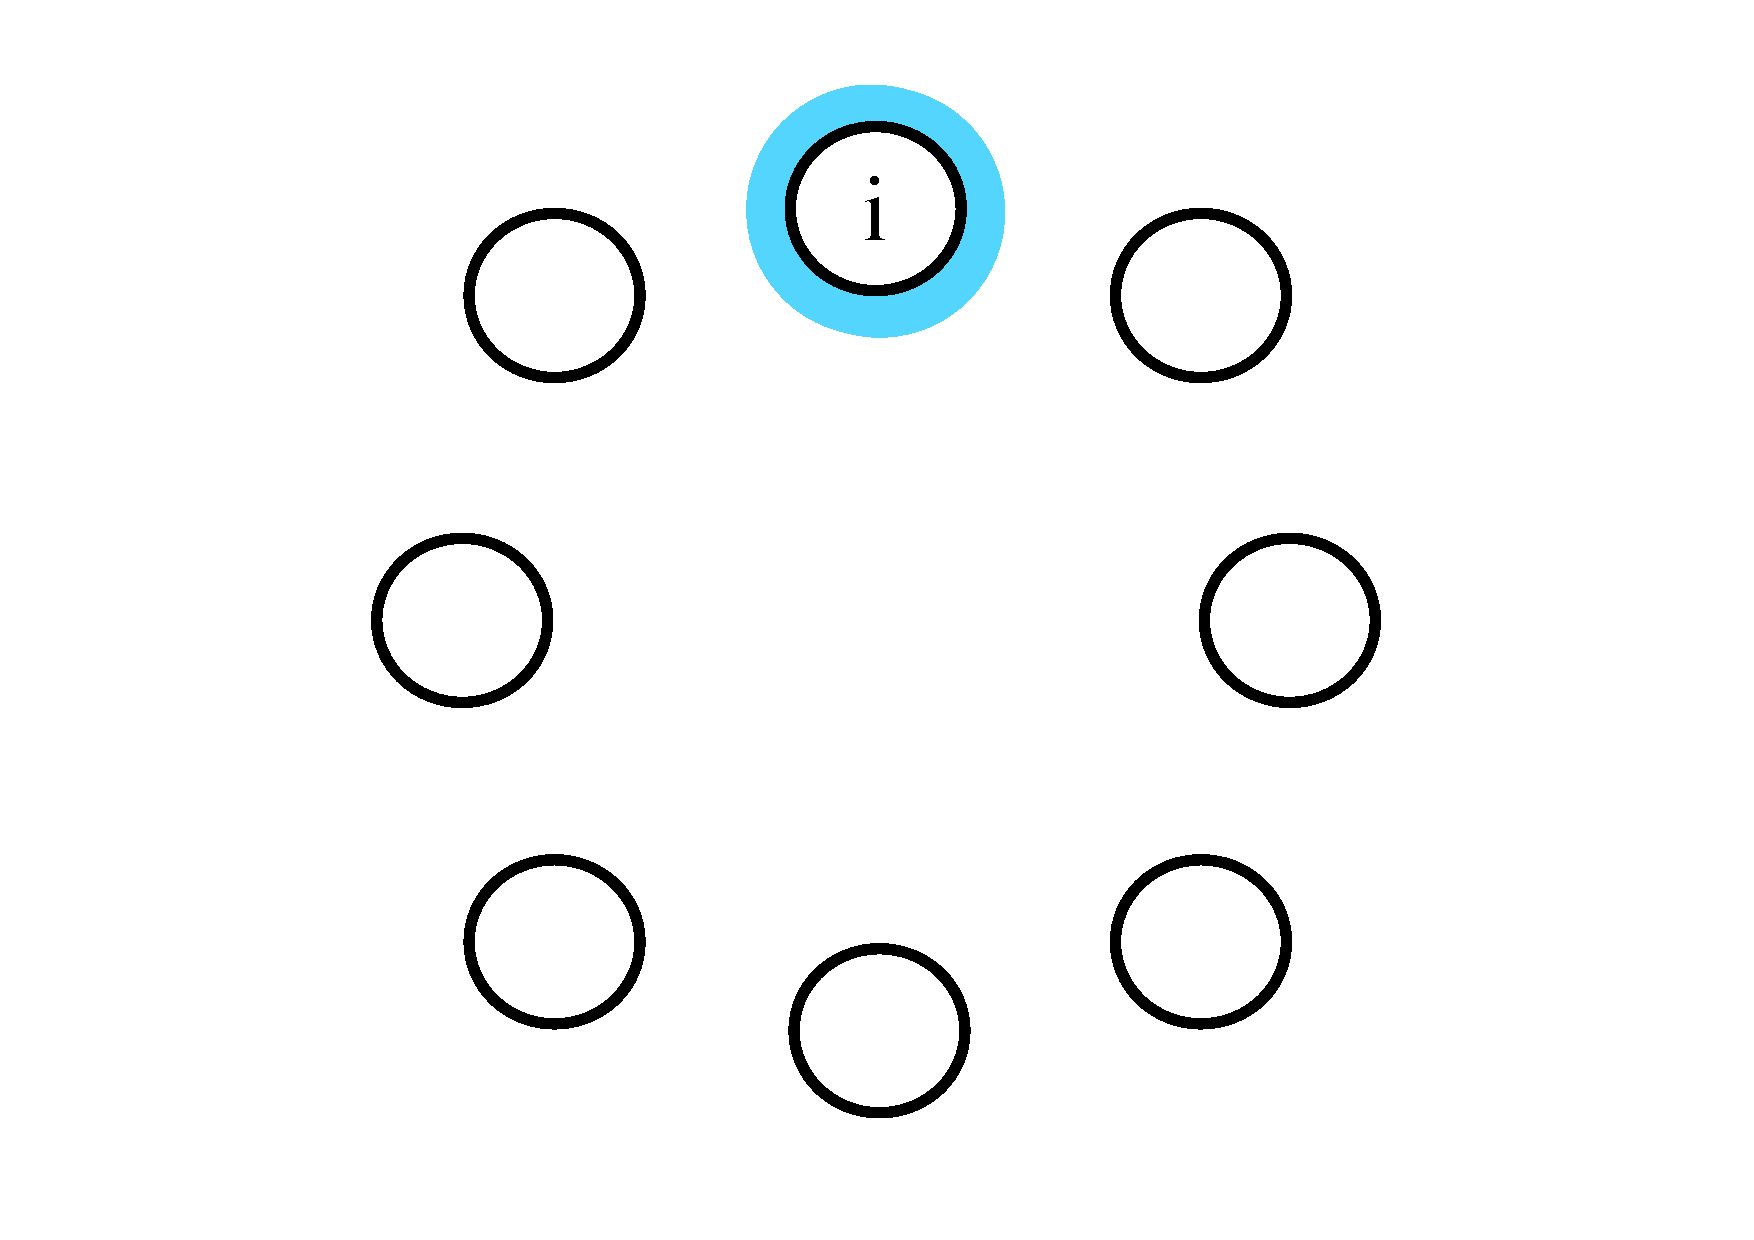
\includegraphics[width=3.8cm]{./figures/fig-24.pdf}
\label{fig:dvms_pte_1}}
%
\subfigure[]{
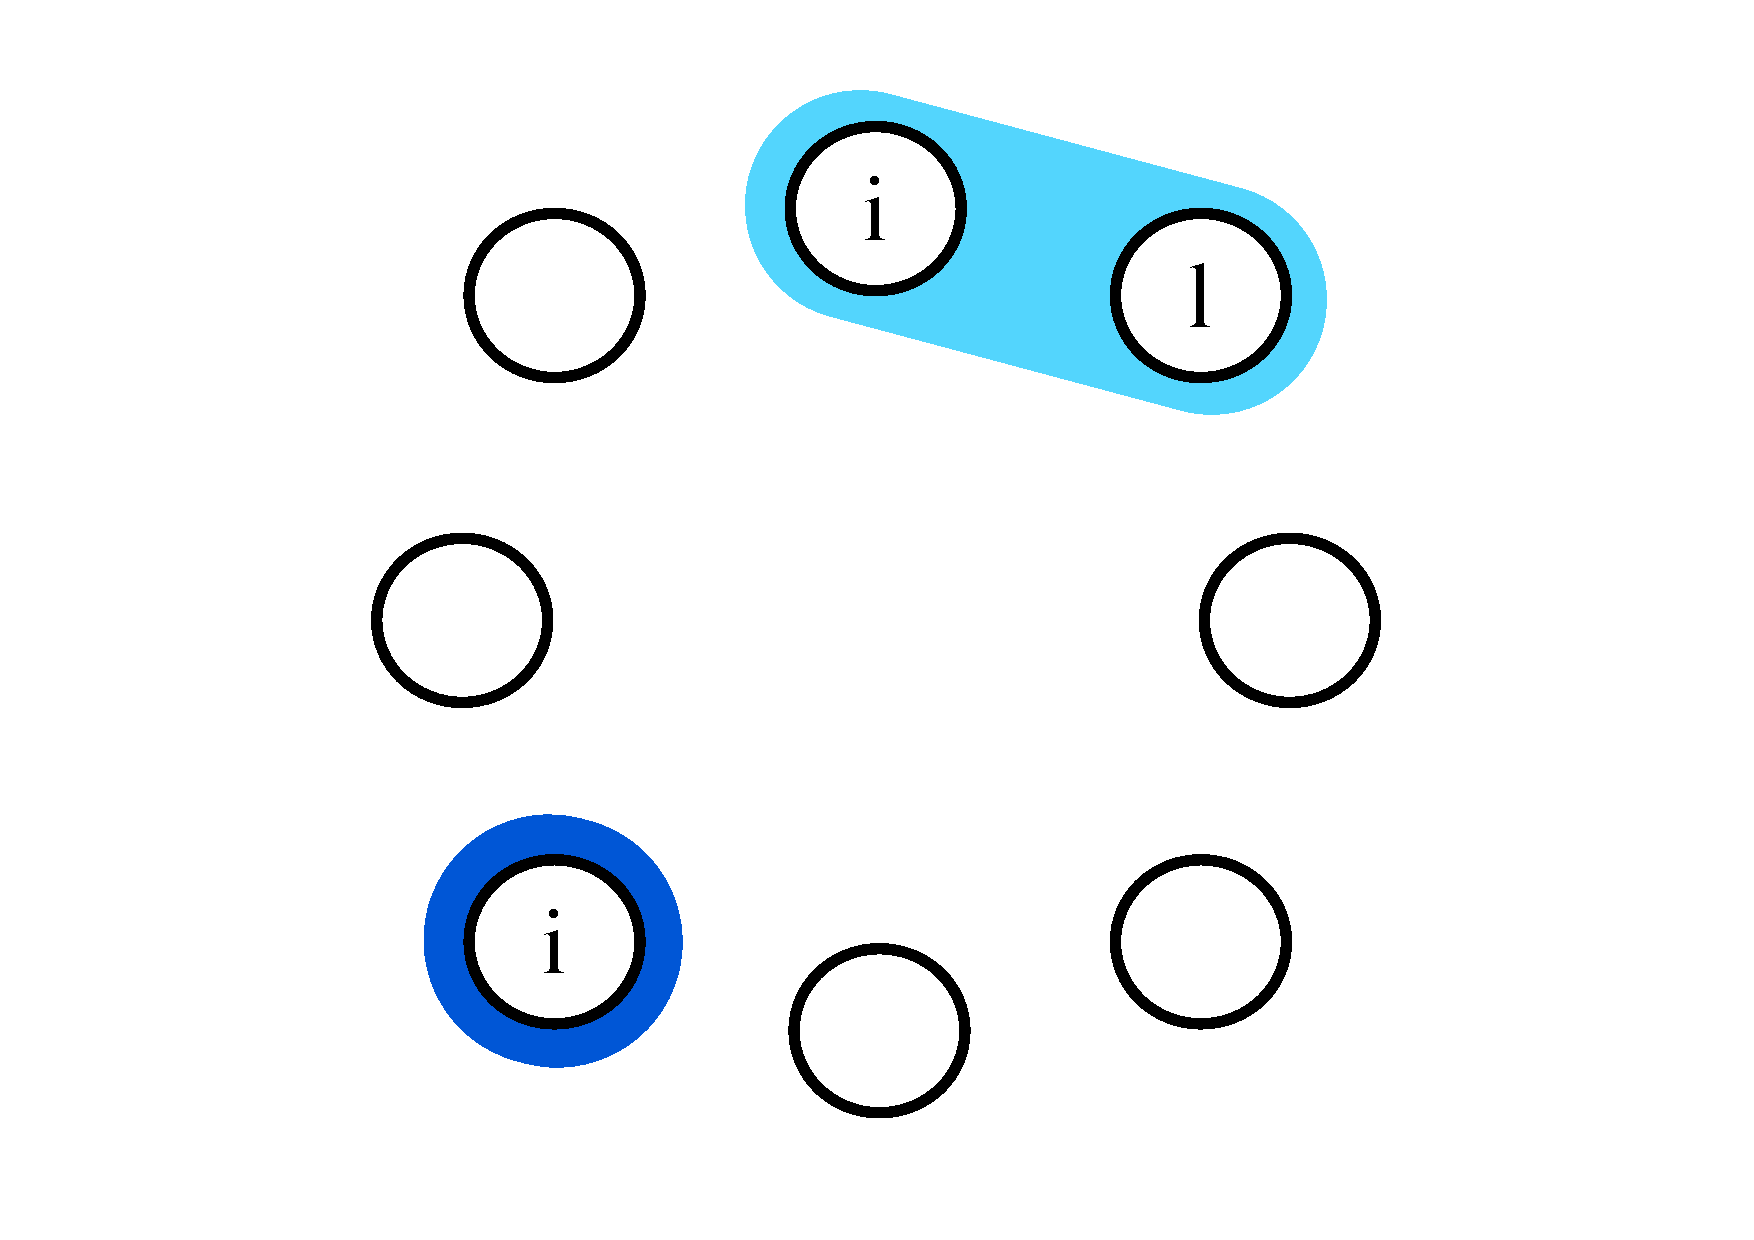
\includegraphics[width=3.8cm]{./figures/fig-25.pdf}
\label{fig:dvms_pte_2}}
%
\subfigure[]{
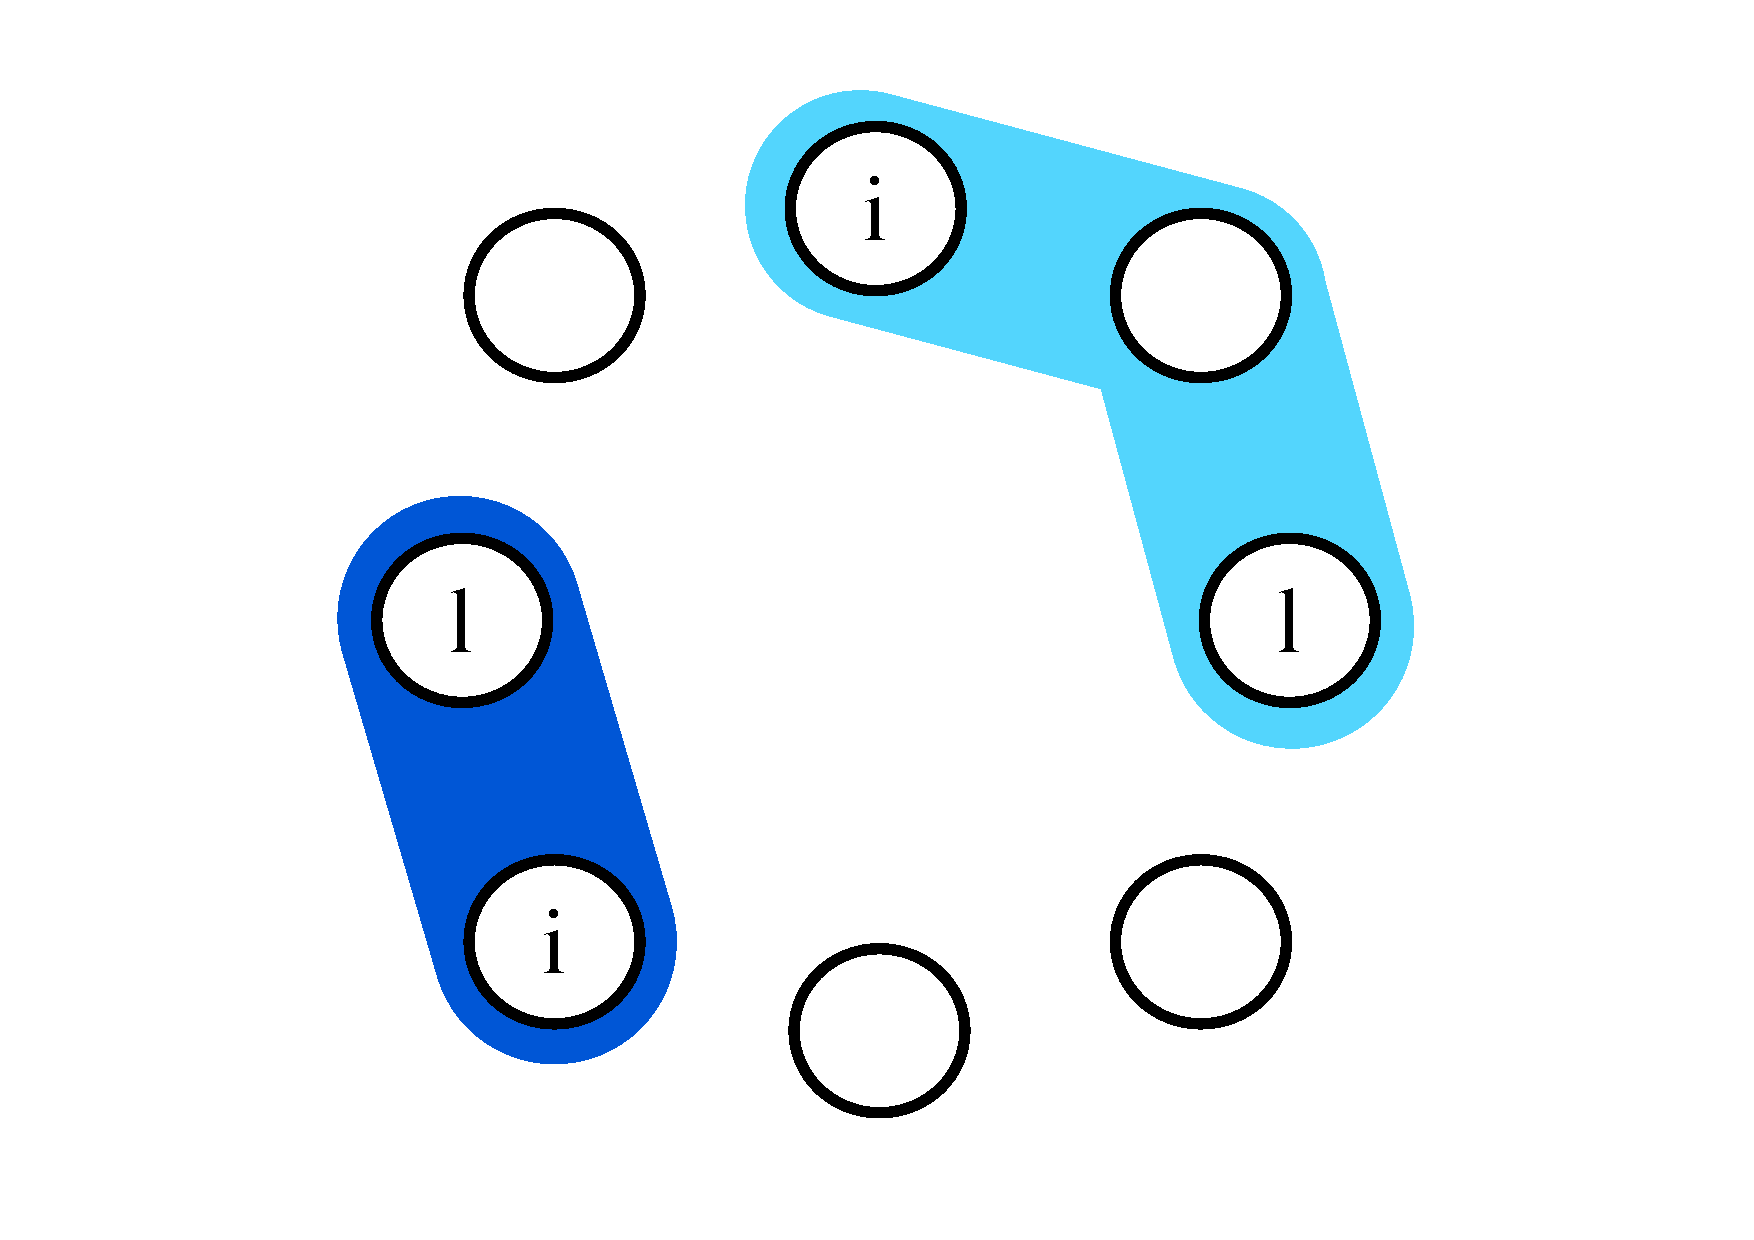
\includegraphics[width=3.8cm]{./figures/fig-26.pdf}
\label{fig:dvms_pte_3}}
%
\subfigure[Legend]{
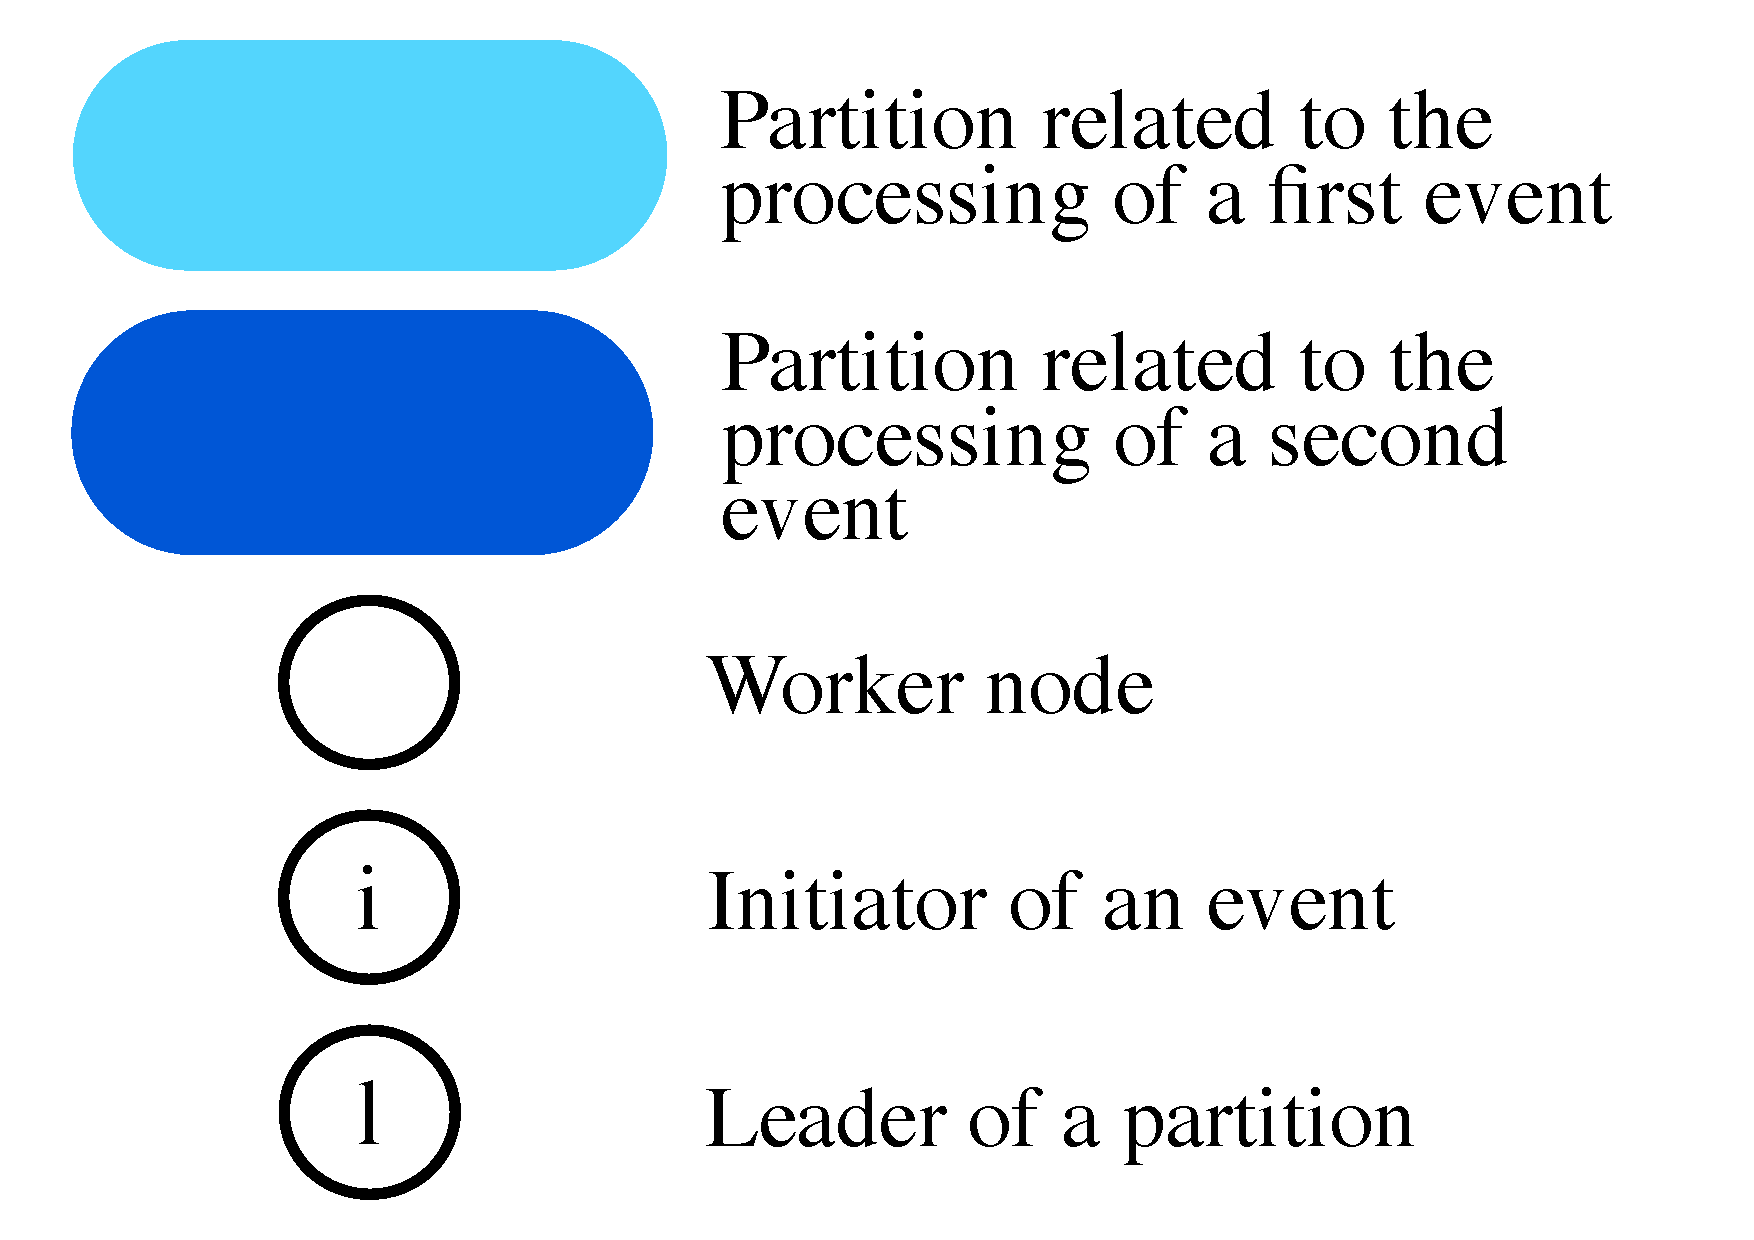
\includegraphics[width=3.8cm]{./figures/fig-27.pdf}
\label{fig:dvms_pte_4}}
%
\caption{Processing two events simultaneously\label{fig:dvms_pte}}
\end{figure}


\subsubsection{Fault-tolerance}

The original implementation of DVMS was not fault-tolerant.


\paragraph{Repairing the Ring.}

Making DVMS fault-tolerant implied first to make the ring fault-tolerant.
Previously, if a node \emph{N\(_{\textit{i}}\)} crashed, an event passing through
node \emph{N\(_{\textit{i-1}}\)} could not reach node \emph{N\(_{\textit{i+1}}\)}.

To preserve the integrity of the ring, we used the algorithms
designed for Chord~\cite{stoica:2001:sigcomm01}.
%
The main idea is to let each node know not only its neighbor, but also its
2\(^{\textit{1}}\) successor, its 2\(^{\textit{2}}\) successor, and so on until the
2\(^{\textit{i}}\) successor, \emph{i} being specified by the administrator;
%
when some part of the ring crashes, network communications can still be
performed by passing through a known alive successor.


\paragraph{Destroying a Partition If One of Its Node Fails.}

Having a fault-tolerant ring was not enough; it was also necessary to make the
problem solving procedure fault-tolerant.

Previously, if the leader of a partition crashed, the problem identified by the
initiator would never be solved; moreover, the nodes of this partition would
remain reserved indefinitely and would not be able to take part to other problem
solving procedures.

To avoid these issues, DVMS now relies on a timeout.  Each node involved in a
partition periodically checks whether the state of its partition changed
recently (for instance, a new node joined the partition).
%
If the state does not change anymore, it probably means that the problem solving
procedure is stuck (maybe because the leader crashed).
%
In this case, each node decides to leave the partition and becomes free to take
part to other problem solving procedures.
